\documentclass[english]{cccconf}
%\documentclass[usemulticol,english]{cccconf}
\usepackage[comma,numbers,square,sort&compress]{natbib}
\usepackage{epstopdf}
\usepackage{amsmath}
\usepackage[linesnumbered,boxed,ruled,commentsnumbered]{algorithm2e}
\usepackage{tabularx}
\usepackage{diagbox}
\usepackage{graphicx}
\usepackage{pdfpages}
\usepackage{subfigure}
\usepackage{amssymb}
\usepackage{amsmath}
\usepackage{xparse}
\usepackage{verbatim}
\usepackage{tikz}
\usepackage{color}
\usepackage[colorlinks,
            linkcolor=black,
            anchorcolor=blue,
            citecolor=blue]{hyperref}
\usepackage{leftidx}
\usepackage{booktabs}
\usetikzlibrary{calc}
\usetikzlibrary{arrows}
\usetikzlibrary{shapes.geometric,positioning}
\usetikzlibrary{3d}

%\usepackage[active,tightpage]{preview}
\DeclareMathOperator*{\argmax}{argmax}
\DeclareMathOperator*{\argmin}{argmin}

\begin{document}

 \title{Extrinsic Calibration of Camera and 3D Laser Sensor System}
 \author{Jingfeng Sui, Shuo Wang}
 \affiliation{Institute of Automation, Chinese Academy of Sciences, Beijing 100190, P.~R.~China\email{suijingfeng2014@ia.ac.cn}}

\maketitle

\begin{abstract}
Robots are typically equipped with multiple complementary sensors such as cameras and laser range finders.
Camera generally provides dense 2D information while range sensors give sparse and accurate depth information
in the form of a set of 3D points.
In order to represent the different data sources in a common coordinate system, extrinsic calibration is needed.
This paper presents a pipeline for extrinsic calibration a zed setero camera with Velodyne LiDAR puck
using a novel self-made 3D marker whose edges can be robustly detected in the image and 3d point cloud.
Our approach first estimate the large sensor displacement using just a single frame.
then we optimize the coarse results by finding the best align of edges in order to obtain a more accurate calibration.
Finally, the ratio of the 3D points correctly projected onto proper image segments is used to evaluate the accuracy of calibration.
\end{abstract}

\keywords{extrinsic calibration, edges extraction, sensor fusion}

\section{Introduction}
Extrinsic calibration is the process of estimating the rigid-body transformation between two or more sensors.
When the camera and the laser are properly calibrated, laser measurements can be correctly projected onto the camera
image, and thus laser points can be associated with color information. Conversely, pixels in the camera image can be
given depth values by querying the nearest laser returns.
It's also a essential steps of 3D Object detection \cite{Premebida2014}\cite{Held2012},
3D tracking\cite{Held2014}, odometry and mapping \cite{Bok2013}.
Methods of the extrinsic calibration of camera with the laser sensor can be classified mainly into two groups.

The first groups of the existing algorithms require a checkerboard like pattern be observed by the sensors from multiple views,
as shown in~Fig.~\ref{fig:PlaneChessboard}. In those methods, the fact that 3D laser points must lie on the calibration plane is
used to form the constrain on the relative position and orientation of the camera coordinate and the laser coordinate,
extrinsic parameters are generally estimated by minimizes a reprojection error.
Zhang is probably the first publish a toolkit for extrinsic calibration of camera and a 2D laser range finder \cite{Zhang2004},
where normals of the checkerboard surface form a non-linear optimization problem that is solved for the extrinsic calibration parameters.
Shortly thereafter, Unnikrishnan presents a method addressing extrinsic calibration of camera and a rotating 2D scanners, and
an initial estimate for the iterative minimization is determined based on a simplified linear least-squares method \cite{Unnikrishnan2005}.
Nunnez modified Zhang's method to perform the extrinsic calibration between a camera and a laser range finder mounted on pan and tilt systems
by observing a checkerboard pattern with the aid of motion obtained by Inertial Measurement Unit \cite{Nunez2009}.
Based on Bouguet's camera calibration toolbox for matlab\footnote{http://www.vision.caltech.edu/bouguetj/calib\_doc/index.html} and Zhang's work,
Kassir provided a realible laser line-segments classify procedure for the calibration which eliminate the effort of manual intervention \cite{Kassir2010}.
Geiger present a toolbox with web interface for calibrate camera to range sensor
using a single view of multiple chessboard patterns placed across a room \cite{Geiger2012}.
Extrinsic calibration using self-made target can also be concluded in this group, see \cite{Rodriguez2008}\cite{He2012}.

\begin{figure}
  \centering
  \label{fig:VelZedSetUp}
  \subfigure
  {
    \label{fig:experiment:a} 
    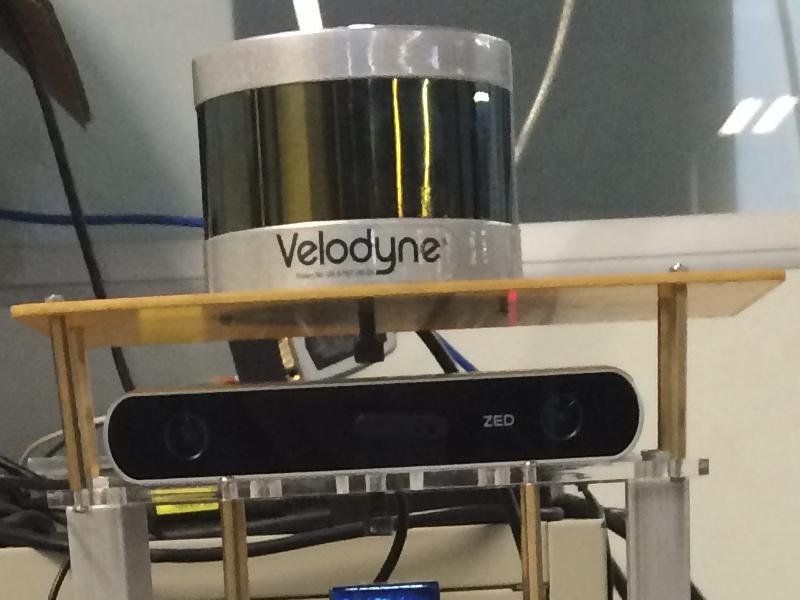
\includegraphics[width=0.22\textwidth]{fig/sensor.JPG}
  }
  \hspace{0.001\linewidth}
  \subfigure
  {
    \label{fig:experiment:b} %% label for second subfigure
    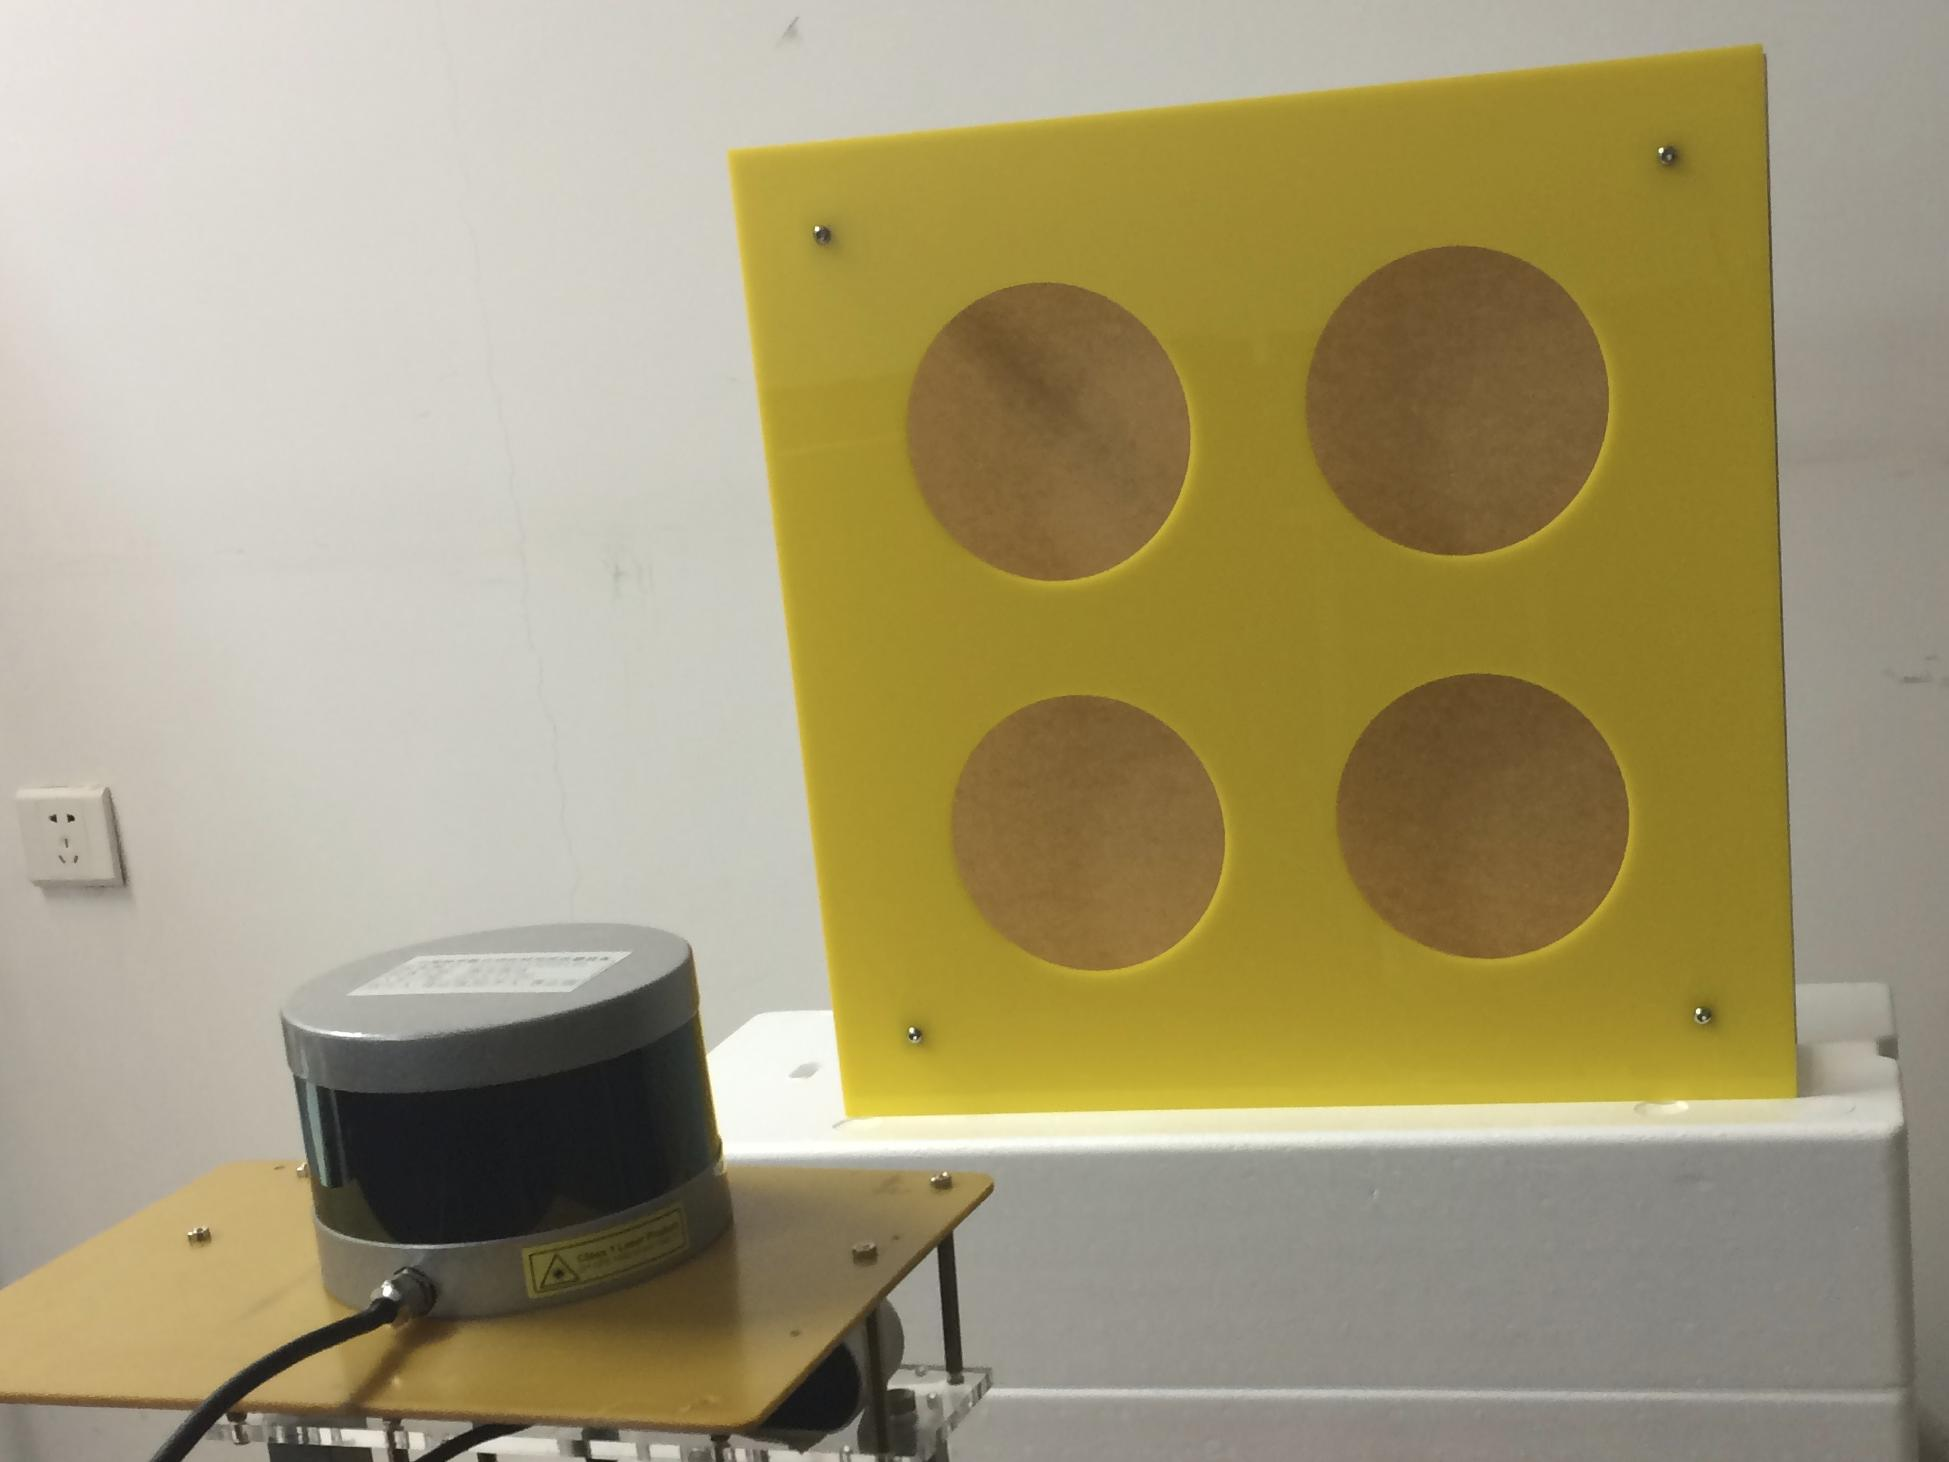
\includegraphics[width=0.22\textwidth]{fig/experimentSmall.JPG}
  }
  \caption{Extrinsic calibration setup for ZED stereo camera with Velodyne 3D LiDAR Puck(we call it VLP16 hereafter)
  which provides 16 lasers rotating around a vertical axis in inclinations
  ranging from $-15^{\circ}$ to $15^{\circ}$, approximately $2^{\circ}$ angular resolution.}
\end{figure}

%distance measurements $360^{\circ}$  horizontally and $30^{\circ}$ vertically


A ��convenient�� calibration method would require no marker, no further hardware requirements but provides sufficient results.
There is a mount of work deal with markerless scenes appears,
which still assuming some features(points, line) are shared by both the camera image and the 3D laser point cloud.
Scaramuzza et al. proposed a technique for the calibration of a 3D laser scanner and omnidirectional camera
by manually established correspondence of extracted features from the laser and the image,
the calibration parameters were calculated by perspective-from-n-points algorithm \cite{Scaramuzza2007}.
Moghadam et al. proposed a method that exploits the linear features present in a typical indoor environment\cite{Moghadam2013},
In this work, the 3D line features extracted from the point cloud and the corresponding 2D line segments extracted from the camera images are used to constrain the rigid-body transformation between the two sensor coordinate frames.
Levinson and Thrun use a series of corresponding laser scans and camera images of arbitrary scenes to automatically estimate the calibration parameters, their objective function based on the matching depth discontinuities detected in laser points cloud and edges detected in images \cite{Levinson2013}.
The techniques that use mutual information as the measure of statistical dependence between the LiDAR and camera sensor modalities for calibration is almost simultaneously proposed by \cite{Pandey2012}, \cite{Taylor2012}.
Pandey and Mcbride calibrate a velodyne-camera system by maximizing the mutual information between laser reflectivity and the image.
The optimization is done by the steepest gradient ascent algorithm.
Taylor and Nieto's work show that maximizing mutual information is better than
minimizing joint entropy of the reflectivity and intensity values obtained from these sensors.
Other methods such as motion based can be found at \cite{Taylor2015}, \cite{Napier}.


Extrinsic calibration of VLP16 with a perspective camera still absence literature can be refer
although aforementioned works do the similar things with this task.
Since 3D point cloud getting from VLP16 is much sparse than HDL64 uesd in the work of \cite{Pandey2012, Taylor2015, Levinson2013},
methods presented in the those works cannot be applied directly to solve extrinsic in our sensor system.

In this paper, we try to close this gap by extended the works of \cite{Velas2014}
to achieve the extrinsic calibration of VLP16 with ZED stereo camera.
The remain work of this paper is organized as follow:
Section 2 give a brief description of our self-made 3D marker.
Section 3 describes the basic constrains from observing the 3D marker, formalizes the problem we are going to solve.
Section 4 discuss the techniques which significantly improve the robustness and accuracy of the calibration 
and provides the corresponding experimental results.

%A modest comparison of proformance and accuracy is conducted.

\section{3D marker description}
We deviced a simple but multifunctional 3D marker which are fixed by four aluminum profiles with each lengths of 20cm.
A checkerboard is attached to the back side of the 3d marker for intrinsic calibration of the camera and
four circular holes with a radius of $R_{circle} = 8.25cm$ are made on the front plane of the 3d marker,
see Fig.~\ref{fig:CalibrationBoard}.
As velodyne-like sensor scans the surrounding environment in horizontally rings,
horizontally oriented edges can not be easily detected when the sensor is mounted as shown in Fig.~\ref{fig:VelZedSetUp}.
Thus we choose the circle as edges so that both the horizontal and the vertical position of the circles can be detected by
VLP16. Note that different colors are chose for the front plane and back plane deliberately.
In theory, black and white are the best candidate color for easier edge detection in camera images.
\begin{figure}[!htb]
  \centering
  \label{fig:CalibrationBoard}
  \subfigure[Front plane]
  {
    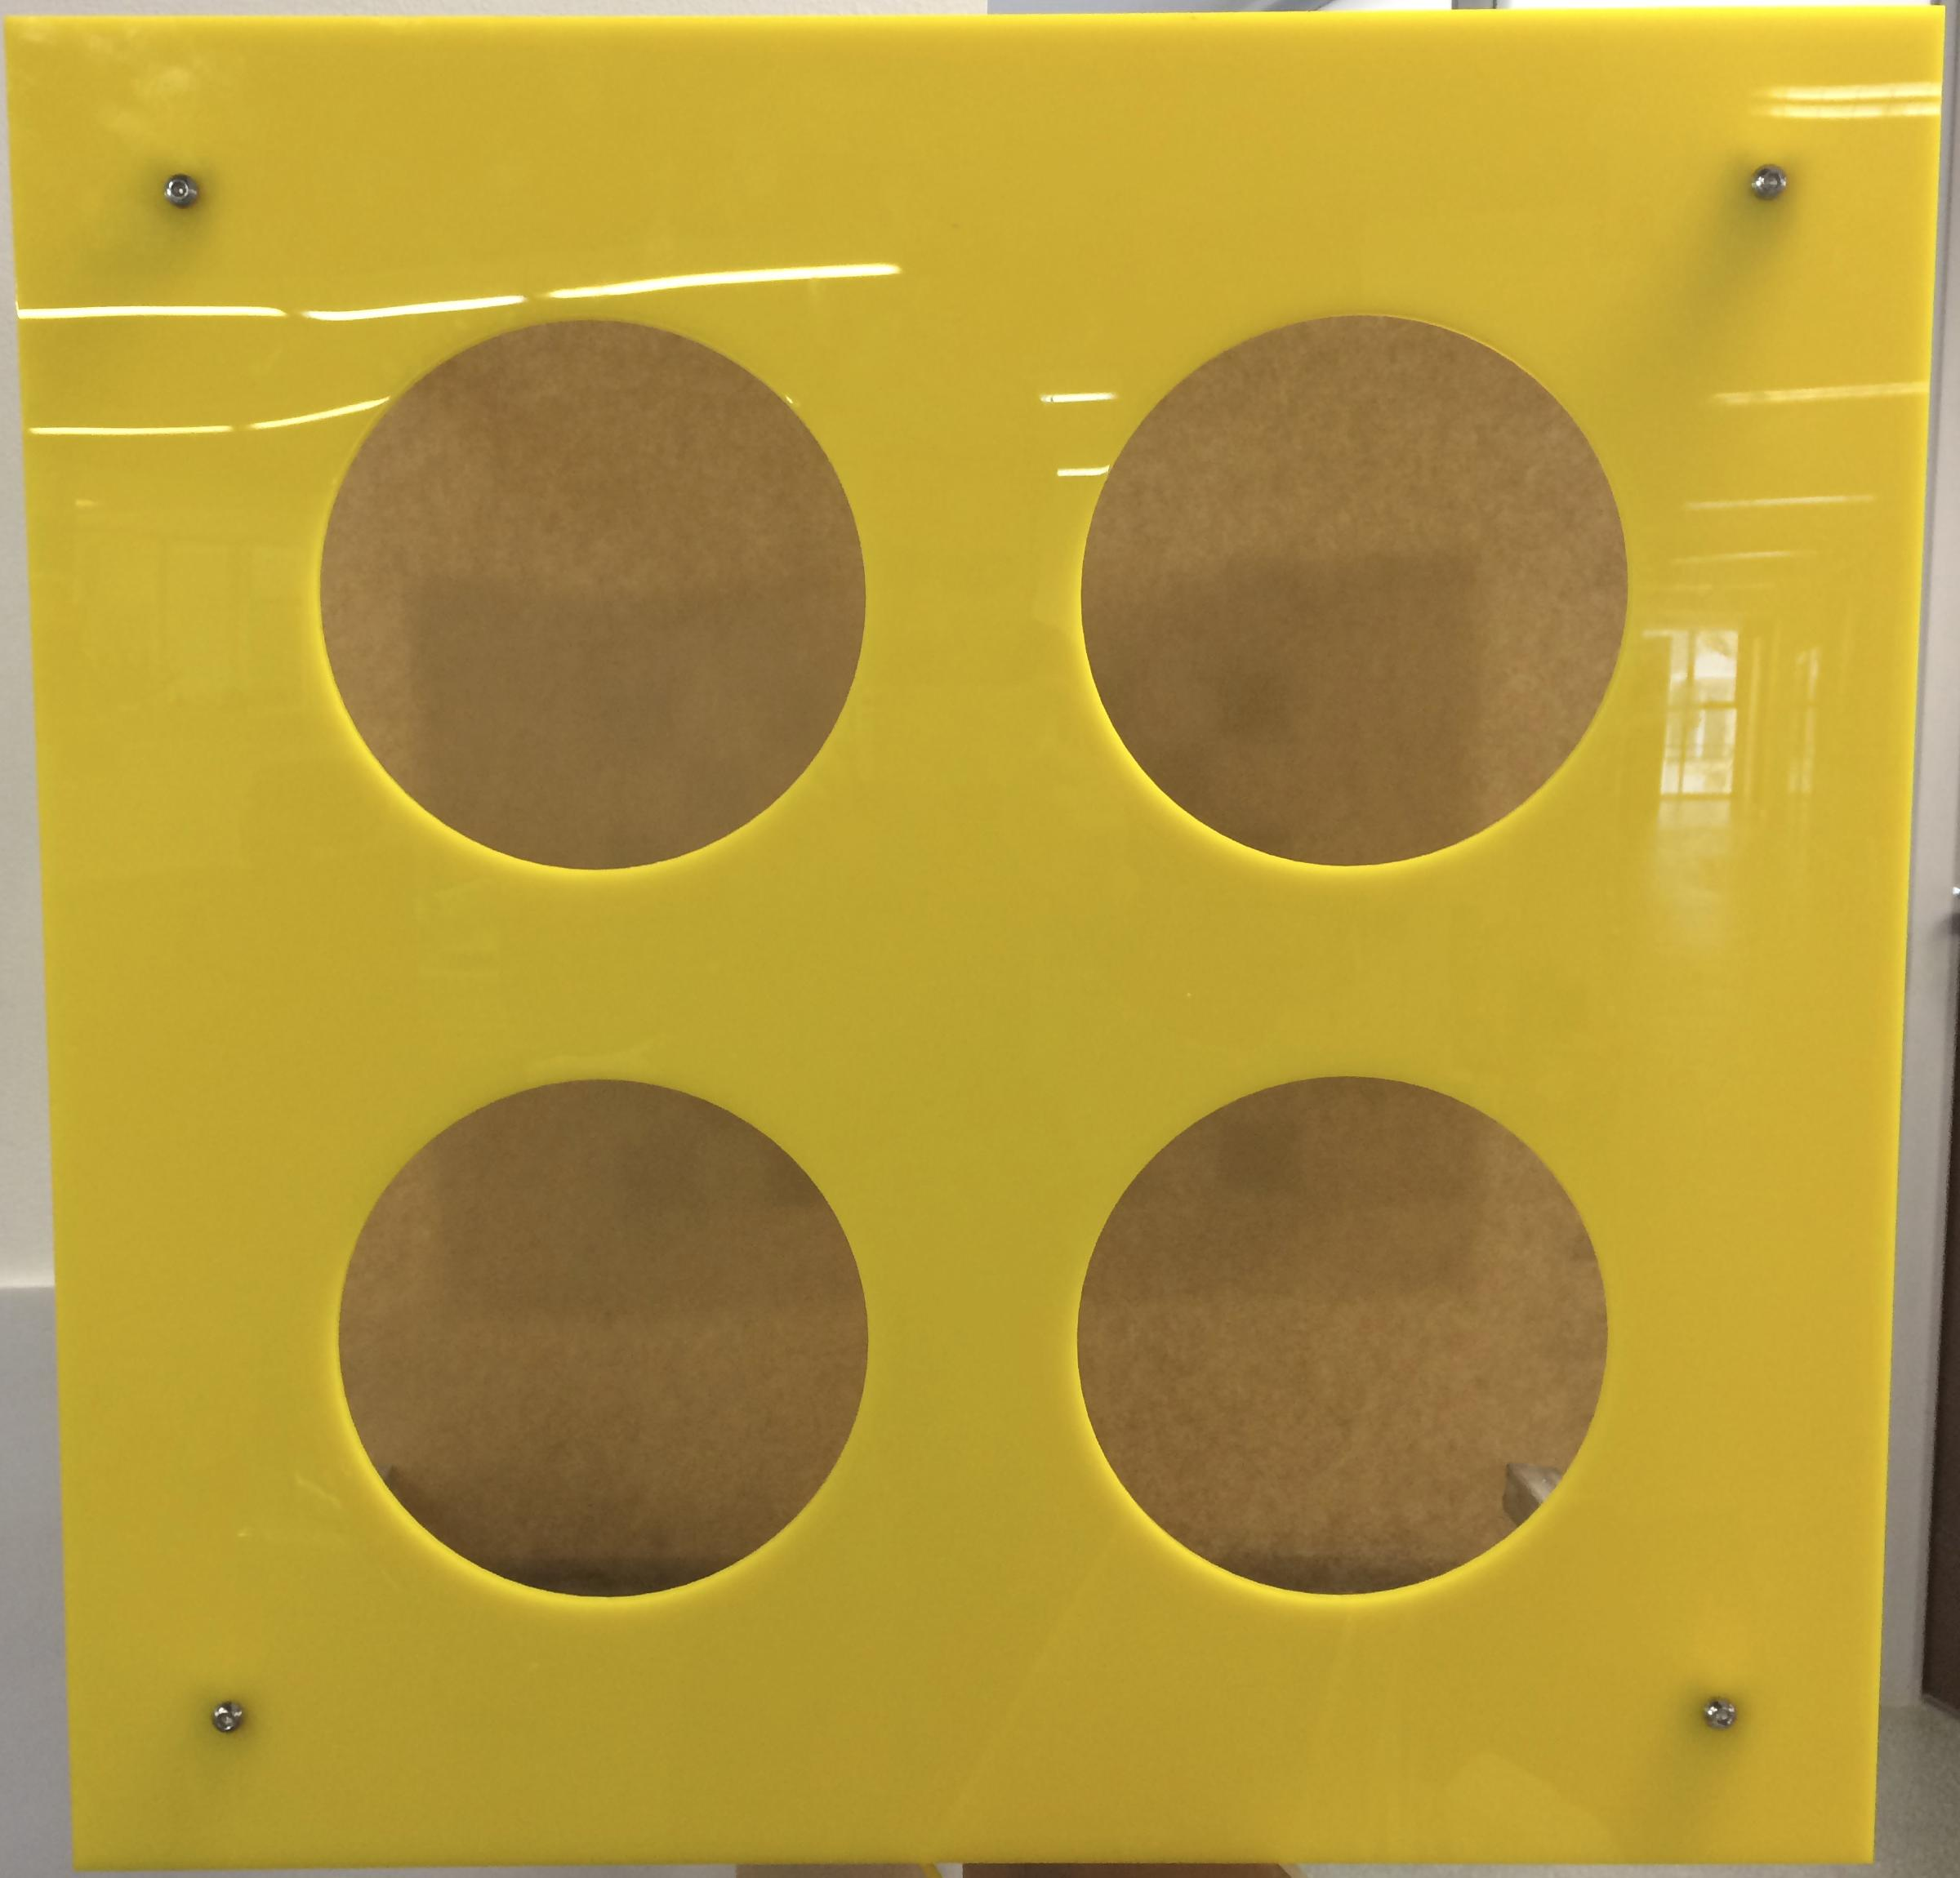
\includegraphics[width=0.18\textwidth]{fig/calibrationBoardFrontSmall.JPG}
  }
  \hspace{0.001\linewidth}
  \subfigure[Back plane]
  {
    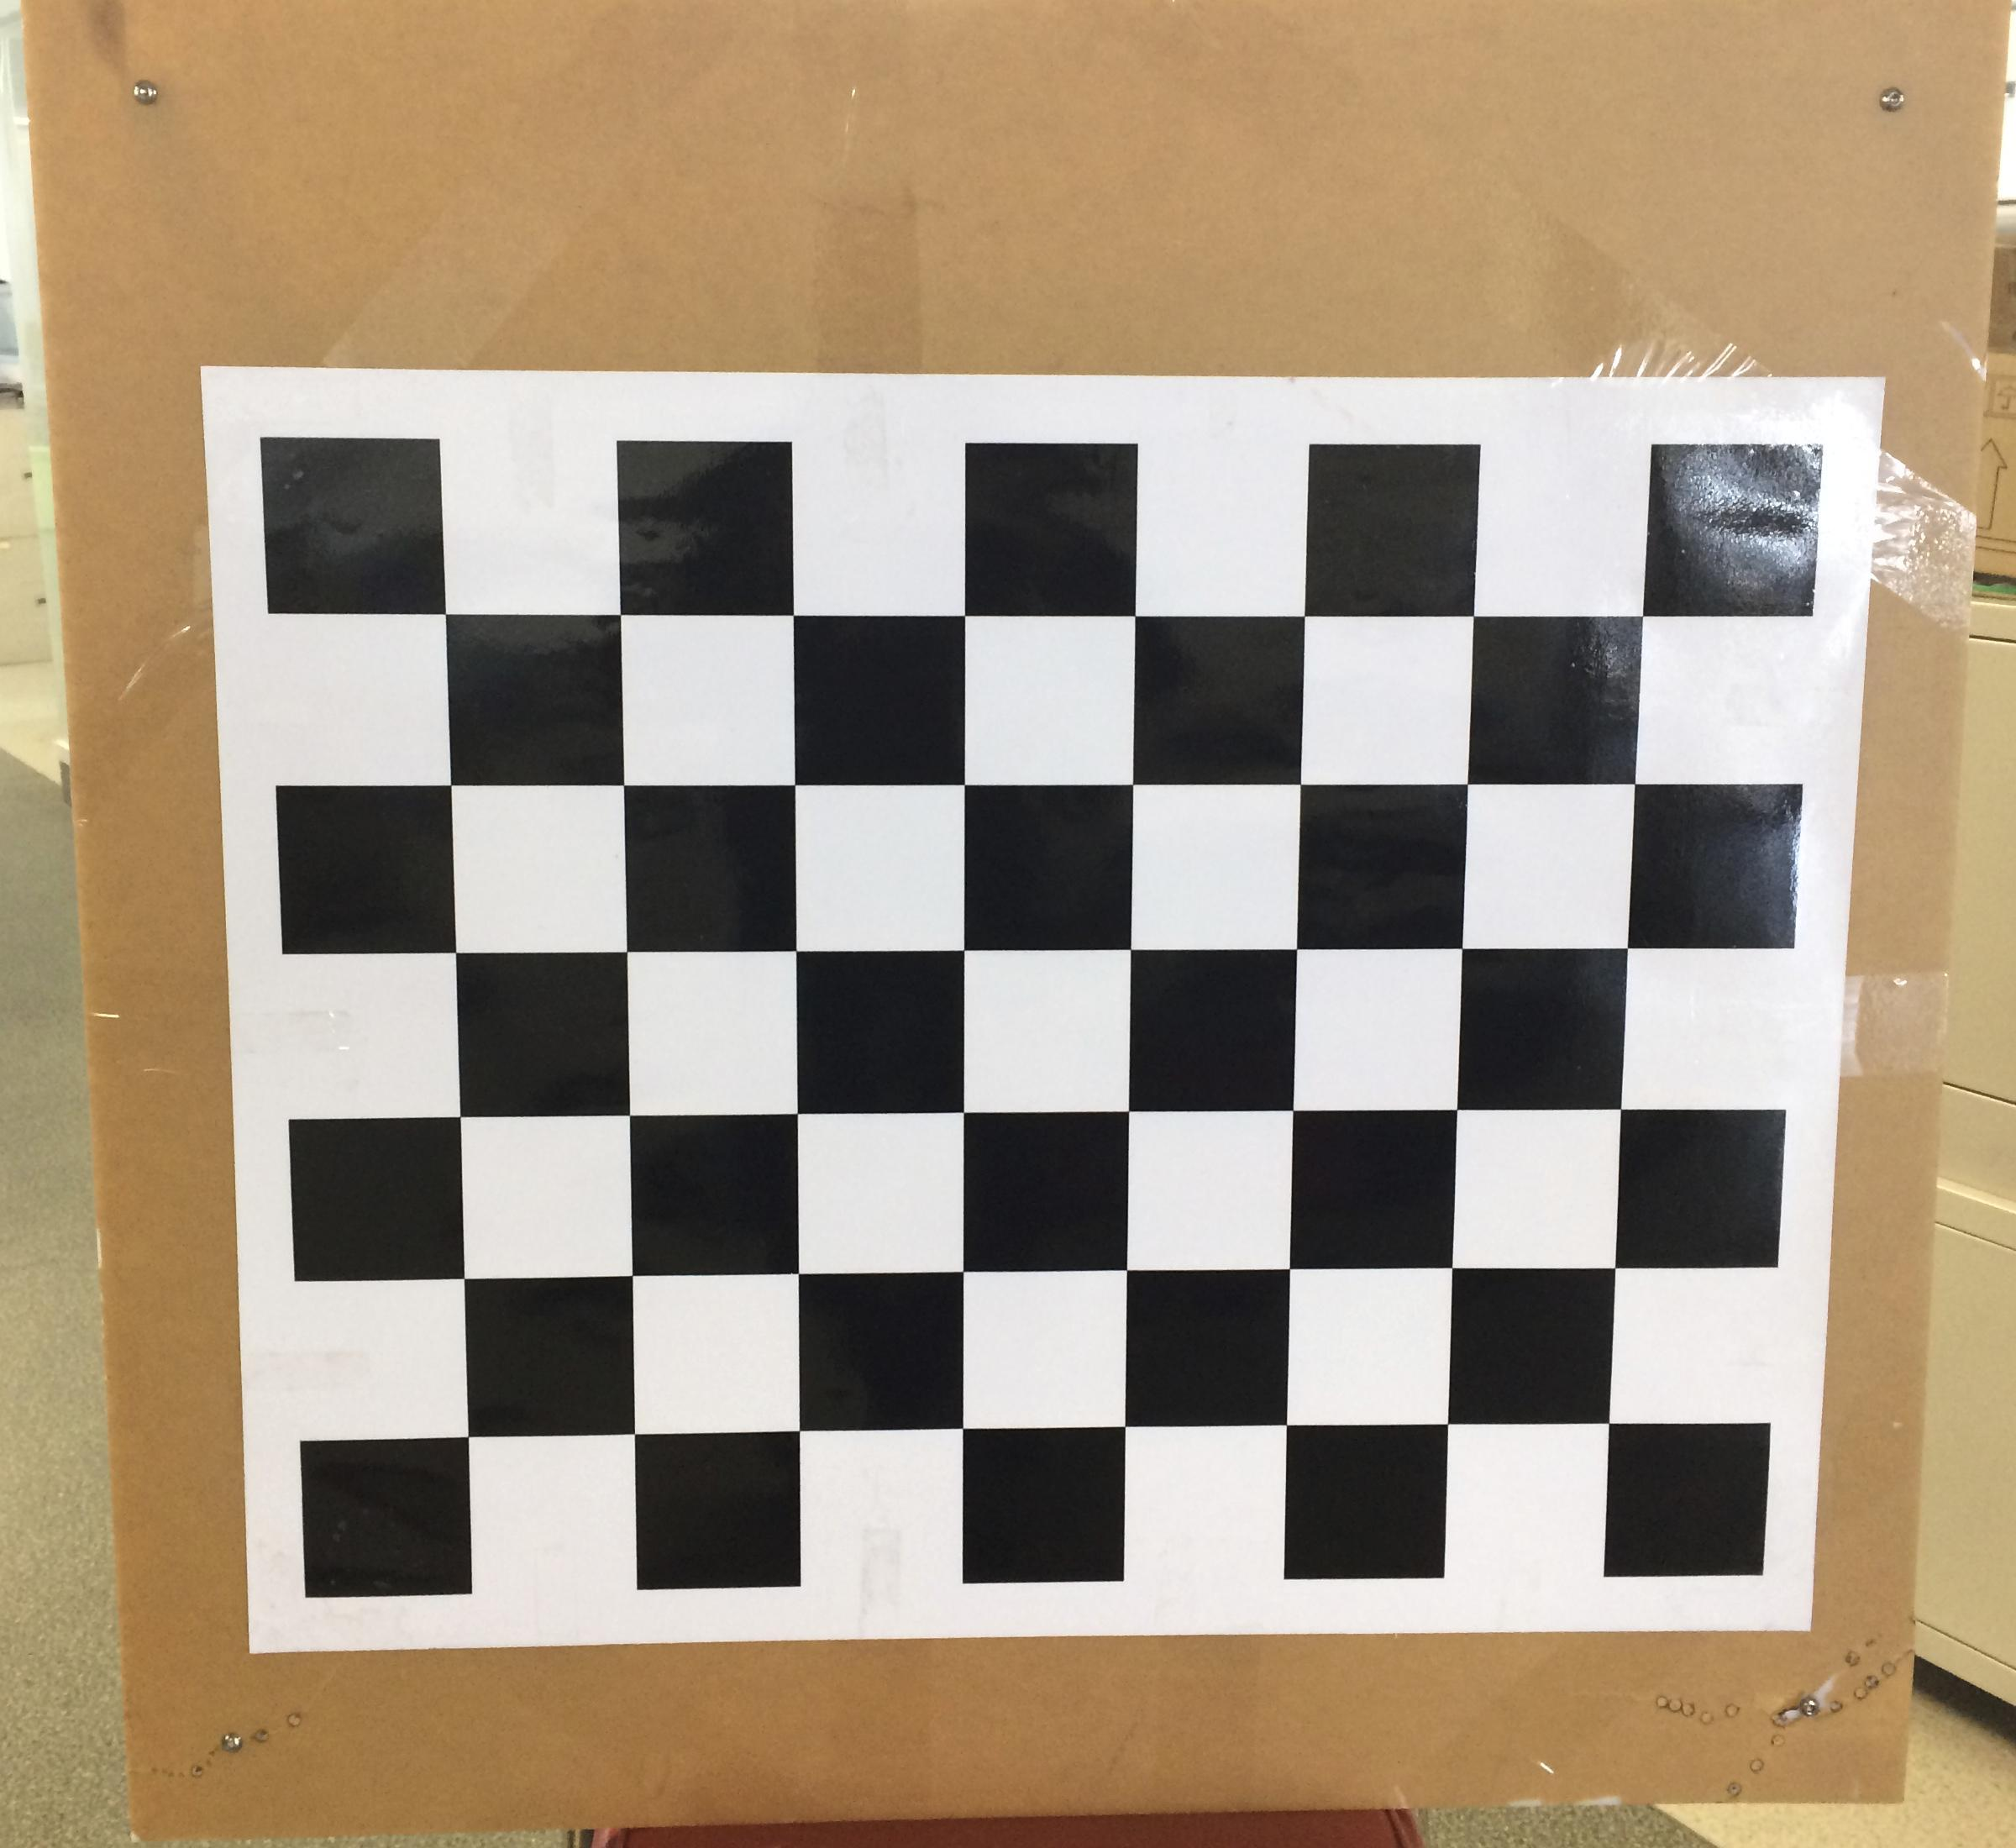
\includegraphics[width=0.19\textwidth]{fig/calibrationBoardBacksmall.JPG}
  }
  \caption{Our 3D marker with four circles of same geometrical on its front side and
  a chessboard is attached its other side used for camera calibration.}
\end{figure}


\section{Methodology}

We propose a two-stage estimation process.
In stage I, a rough translation between two sensor is estimated
using the four pairs circle centers as the corresponding points in image and point cloud.
In this stage, the coordinate axis of VLP16 should be approximately aligned with axis of image coordinate.
but not require very precise as long as the relative rotation is small,
as shown in our sensor systems configurations(Fig.~\ref{fig:VelZedSetUp}).
The result of this stage is used as initialization for the stage II which
calibration of sensors including the rotation is refined by maximized the edge similarity object function.

\begin{figure}[htpb]
  \centering
  \subfigure[Extrinsic and intrinsic calibration with a chessboard\label{fig:PlaneChessboard}]
  {
    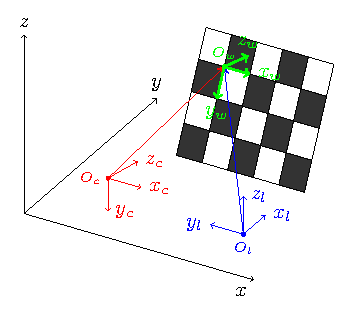
\includegraphics{fig/CalibrationChessboard.pdf}
  }
  \hspace{1em}%
  \subfigure[ Extrinsic calibration with our 3D marker,
  $O_l$ is the default reference frame of the point cloud getted from VLP16,
  $O_c$ denote the image reference frame\label{fig:Plane3DMarker}]
  {
    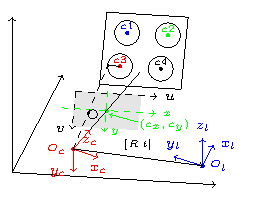
\includegraphics[width=0.35\textwidth]{fig/Calibration3dMarker.pdf}
  }
  \label{fig:SchematicOfTf}
  \caption{A schematic of the calibration problem.
  The goal is to find the rotation $\mathbf{R}$ and the translation $\mathbf{t}$
which transform points in laser coordinate $O_l$ to camera coordinate $O_c$.}
\end{figure}

The left and right camera of ZED used in this paper is modeled with the perspective projection model \cite{ZhangZY200} and
the camera is calibrated before the extrinsic calibration by getting several view of our 3d marker's back side,
the schematic is shown in Fig.~\ref{fig:PlaneChessboard}.
Then we start extrinsic calibration using the front side our 3d marker,
the 3D marker should be placed approximately straight in the front of the camera and the VLP16.
The relationship of between a 3D point $P = [X, Y, Z, 1]$ and its corresponding position in image $p = [u, v, 1]$ is given by
\begin{equation}
s\begin{bmatrix} u \\ v \\ 1 \end{bmatrix} =
C \begin{bmatrix} \mathbf{R} & \mathbf{t} \end{bmatrix} \begin{bmatrix} X \\ Y \\ Z \\ 1 \end{bmatrix},
C = \begin{bmatrix} f_x & 0 & c_x\\ 0 & f_y & c_y \\ 0 & 0 & 1\end{bmatrix}
\label{eq:eq1}
\end{equation}
where $s$ is scale factor, $ C $ is the camera intrinsic matrix,
$(c_x, c_y)$ is the coordinates of the principal point usually at the image center,
Generally $f_x = f_y = f$ are the focal lengths expressed in pixel units.
$ \begin{bmatrix} \mathbf{R} & \mathbf{t} \end{bmatrix}$ is called a matrix of extrinsic parameters.
It is used to describe the rigid transformation a point ${{^l}P}$ represented in the laser frame into ${^c}P$
which is the camera's frame of reference.
\begin{equation}
{{^c}P} = \mathbf{R} {{^l}P} + \mathbf{t}
\label{eq:eq2}
\end{equation}

\subsection{Stage I: Solve the large translation}
In fact, we already have manually measured extrinsic shown in Table~\ref{tab:mannual}.
If we project the edge points extracted in the image, we will get a worse result as shown in Fig~\ref{fig:worse}.
Thus a more accurate extrinsic is needed. To address this problems, an automated and effective method is proposed.
A brief Summary of Stage I is given as follows:
\begin{itemize}
\item[(1)] Detect circles in image, solve the circle's centers $c_I(u_i, v_i), i=1,2,3,4$
and radius $r_1, r_2, r_3, r_4$;
\item[(2)] Detect the circle centers  $c_l(X_i, Y_i, Z_i), i=1,2,3,4$ in the point cloud.
\item[(3)] Estimate the translation between laser frame and the camera frame:
\begin{equation}
t_{zi} = \dfrac{ R_{circle} \cdot f}{r_i} - Z_i\\
\label{eq:LargeTranslationZ}
\end{equation}
\begin{equation}
\begin{array}{c}
t_{xi} = \dfrac{ (u_{i} - o_x) \cdot (Z_i + t_z) }{f} - X_i\\
t_{yi} = \dfrac{ (v_{i} - o_y) \cdot (Z_i + t_z) }{f} - Y_i
\end{array}
\label{eq:LargeTranslationXY}
\end{equation}
\begin{equation}
\hat{t}_z = \dfrac{\sum^{4N}_{i=1}{t_{zi}}}{4},
\hat{t}_x = \dfrac{\sum^{4N}_{i=1}{t_{xi}}}{4},
\hat{t}_y = \dfrac{\sum^{4N}_{i=1}{t_{yi}}}{4}.
\label{eq:LargeTranslationALL}
\end{equation}
\end{itemize}
where $R_{circle}$ is the actual radius of circle in the 3D-marker, $N$ is the number of pair data provided.
The large translation can be roughly estimate using only single pair of the data,
However, using multi pairs of the data will improve the accuracy of calibration.
More details about the techniques we used in the process of calibration is given in the following sections.

\subsubsection{Circles detection on image}

Edges extraction in the point cloud and image is aimed at finding the correspondence points of them.
Assume we are given a series of the camera images $I_{1:n}$ and point clouds $P_{1:n}$ from $n$ view of the 3D marker.
The goal is to find the parameter $R$ and $t$ which best align laser depth discontinuities with image edges.

\begin{equation}
G_x=\begin{bmatrix}-1 & 0 & 1\\-2 & 0 & 2\\-1 & 0 & 1\end{bmatrix}*I,
G_y=\begin{bmatrix}-1 & -2 & -1\\0 & 0 & 0\\1 & 2 & 1\end{bmatrix}*I \\
\end{equation}

\begin{equation}
G = \sqrt{G^2_x + G^2_y}
\end{equation}

\begin{figure}[htbp]
  \centering
  \subfigure[Edge Image $E_I$ \label{fig:subfig:a}]
  {
    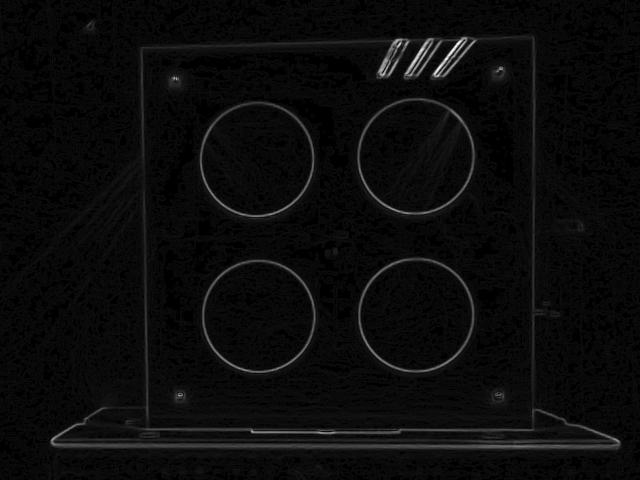
\includegraphics[width=0.22\textwidth]{fig/edgeImg.jpg}
  }
  \hspace{0.01cm}
  \subfigure[Detected circles \label{fig:subfig:b}]
  {
    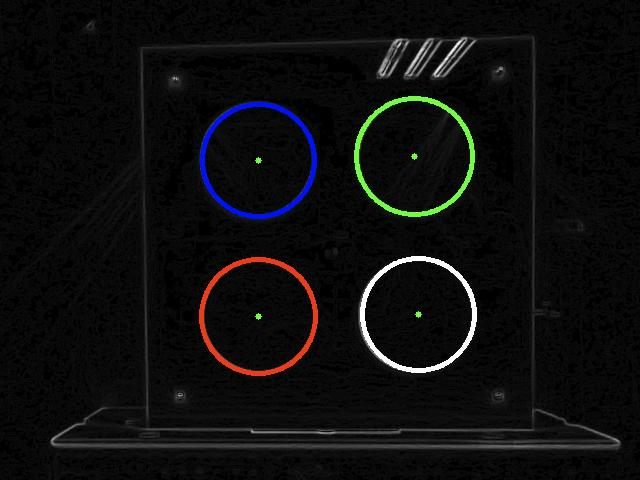
\includegraphics[width=0.22\textwidth]{fig/HoughCircle.jpg}
  }
  \caption{Circles detected in edge image using hough transform\label{fig:HoughCircle}}
\end{figure}
We use a two-step process, first each image is converted to grayscale and creating edge image $E$ using Sobal operator.
Next, The circles are detected in the edge image using the hough gradient method \cite{Yuen1990} which has been implemented in OpenCV,
Fig.~\ref{fig:HoughCircle} show the results.


\subsubsection{Circle detection in point cloud}
Edge detection and feature line extraction in 3D-point clouds have become a novel research topic\cite{Wang2013}.
However, the established edge detection methods defined for images cannot be applied directly to 3D-point clouds.
The main reasons is the data representation is different.
An image contains abundant 2D spectral information and its pixel is organized as a two-dimentional matrix
so that the neighborhood of a pixel can easily be determined
whereas a 3D-point cloud generated by velodyne-like sensors is an irregularly distributed sparse point set,
thus the neighborhood of a point is more complex than that of a pixel in an image.
Fig.~\ref{fig:OriginalPC} gives a view of the multiple rotating beams collected from VLP16.

\begin{figure}[htbp]
  \centering
  \subfigure[Top view]
  {
    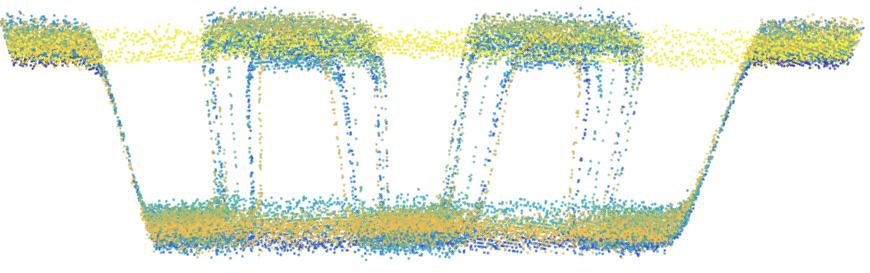
\includegraphics[width=0.4\textwidth]{fig/top_view.jpg}
  }
  \subfigure[Front view]
  {
    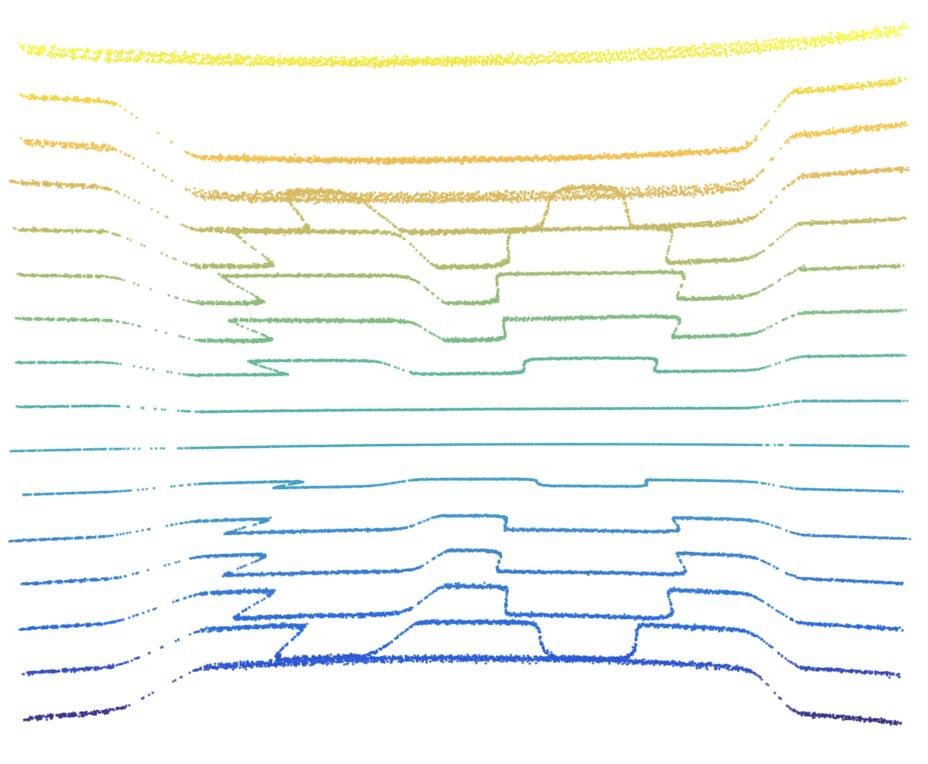
\includegraphics[width=0.4\textwidth]{fig/frontview.jpg}
  }
  \caption{An example of data captured from VLP16.\label{fig:OriginalPC}}
\end{figure}

We combines depth gap metric and RANdom SAmple Consensus (RANSAC)~\cite{RANSAC2000, Mach1981} to detect circles.
In the second step, edges extraction is achieved by detecting the large depth discontinuities for each laser rings independently,
Every 3D points in the laser scan ring is assign a value which depends on the depth measurements of its neighborhoods.
\begin{equation}
I_l(P_i) = \lvert P_{i+2}.z + P_{i+1}.z - P_{i-1}.z - P_{i-2}.z \rvert^\gamma
\label{eq:edgesMetric}
\end{equation}
\begin{equation}
E_l = \{ P_i \lvert I_l(P_{i}) > \delta,\; i = 1,2,\cdots,M.\}
\label{eq:filterEdgesOut}
\end{equation}
where $I_l(P_{i})$ represents the ``edgeness'' of a 3D laser point,
$P_{i}.z$ is the depth of a laser measurement\footnote{Replace $P_{i}.z$ with $P_{i}.r$ will make $P_{i}.I$ larger,
as $P_{i}.r = \sqrt{P_{i}.x^2 + P_{i}.y^2 + P_{i}.z^2}$.
However, by enlarging $\delta$ can achieve the equivalent effect.},
$\gamma$ is a parameter($\gamma >= 1$) use to suppress small distortion of the laser measurements.
The bigger $\gamma$ is, the higher value will be assign to the potential edges points than the distortion.
$\delta$ is a threshold need tuned to select the edge points $E_l$ out, Fig.~\ref{fig:EdgesIn3D} illustrate the result.
In addition, experiment show that edges extracted using formula~(\ref{eq:edgesMetric}) is not very sensitive to minor changes in $\delta$.
\begin{figure}[!htbp]
  \centering
  \subfigure[Edges $E_l$\label{fig:EdgesIn3D}]
  {
     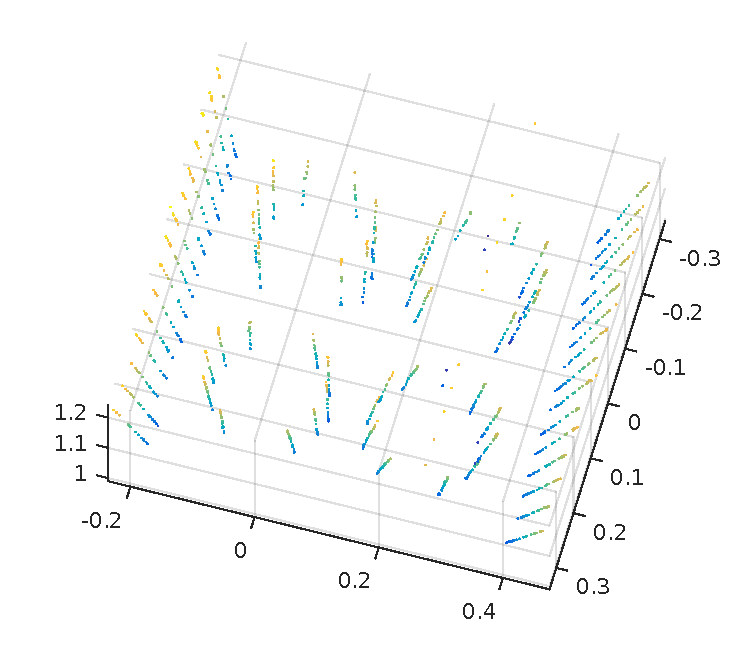
\includegraphics[width=0.23\textwidth]{fig/edge3d.pdf}
  }
  \hspace{0.001cm}
  \subfigure[Front plane inliers \label{fig:FinedPlane}]
  {
    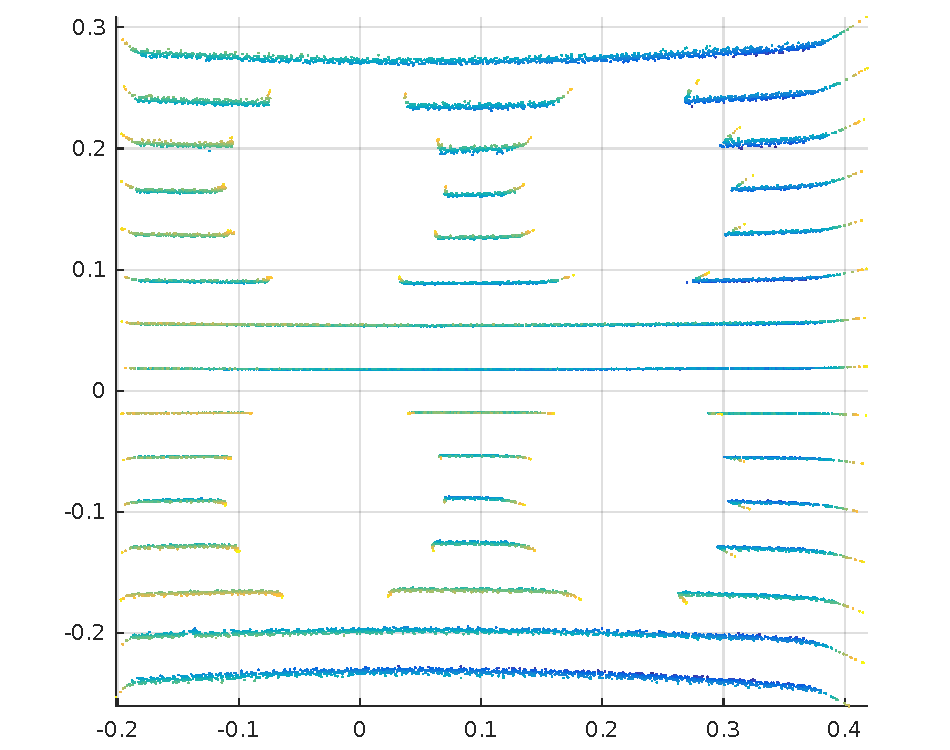
\includegraphics[width=0.22\textwidth]{fig/frontplane.pdf}
  }
  \caption{(a) Edges $E_l$ extracted from the original point cloud using
  formula~(\ref{eq:edgesMetric}) and~(\ref{eq:filterEdgesOut}) with $\gamma = 1.2, \delta = 0.3$.
  (b) the front plane of the point cloud fitting with RANSAC\label{fig:ExtractPlane} algorithm.}
\end{figure}
In the second step, segmentation of the front plane is from the original point cloud is performed using the
RANSAC method implemented in the Point Cloud Library~\cite{Rusu2011}.
The point cloud are first fitted with plane model with a large distance threshold.
Then, the plane is refitted with a small distance threshold so that we can get more accurate front plane model.
RANSAC returns the normalized normals of planes: $(a_f, b_f, c_f)$ and the distance $d_f$ of laser origin to the plane.
\begin{equation}
a_fx+b_fy+c_fz+d_f = 0
\label{eq:frontplanemodel}
\end{equation}
the result is shown in~Fig~\ref{fig:FinedPlane}.

In order to locate the centers robustly,
we force all the edge points $E_l(X_i, Y_i, Z_i)$ project to the front plane, see Fig.~\ref{fig:edgePC}.

\begin{equation}
  \left\{
  \begin{aligned}
    X'_i = - \frac{d_f}{a_f X_i + b_f Y_i + c_f Z_i}\cdot X_i \\
    Y'_i = - \frac{d_f}{a_f X_i + b_f Y_i + c_f Z_i}\cdot Y_i \\
    Z'_i = - \frac{d_f}{a_f X_i + b_f Y_i + c_f Z_i}\cdot Z_i
  \end{aligned}
  \right.
  \label{eq:PerspectiveLaser2Plane}
\end{equation}

\begin{figure}[!htbp]
  \centering
  \subfigure[Project all edges point $E_{p}$ to the fined front plane\label{fig:edgePC} using~(\ref{eq:PerspectiveLaser2Plane})]
  {
    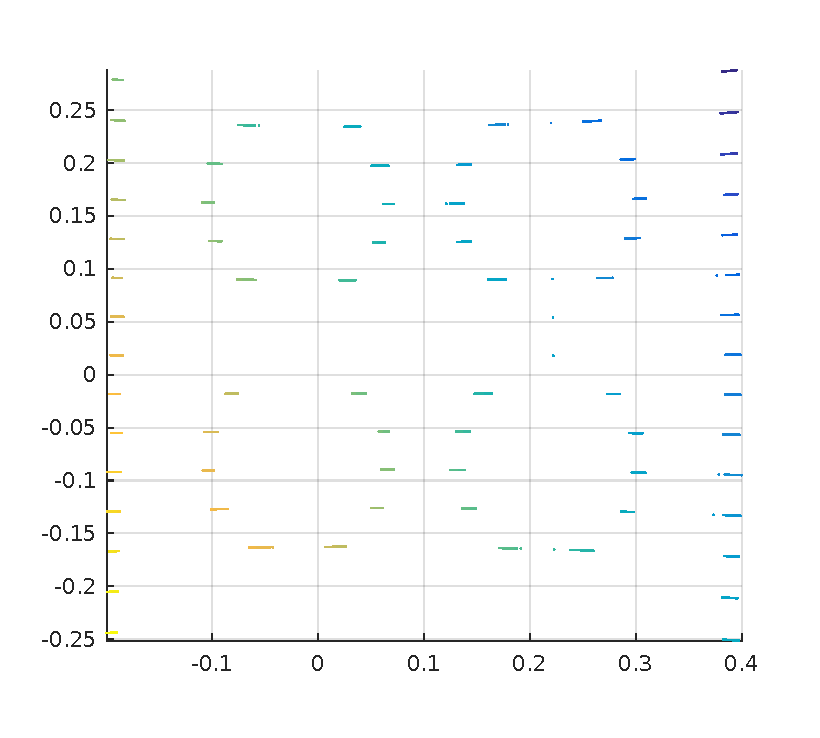
\includegraphics[width=0.44\textwidth]{fig/projecttofrontplane.pdf}
  }
  \subfigure[Four circles extracted\label{fig:circleExtracted}]
  {
    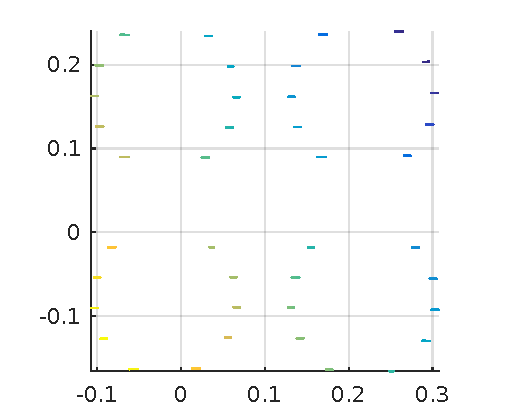
\includegraphics[width=0.24\textwidth]{fig/FourCirclePure.pdf}
  }
  \hspace{0.01cm}
  \subfigure[Removed Lines\label{fig:RemovedLines}]
  {
    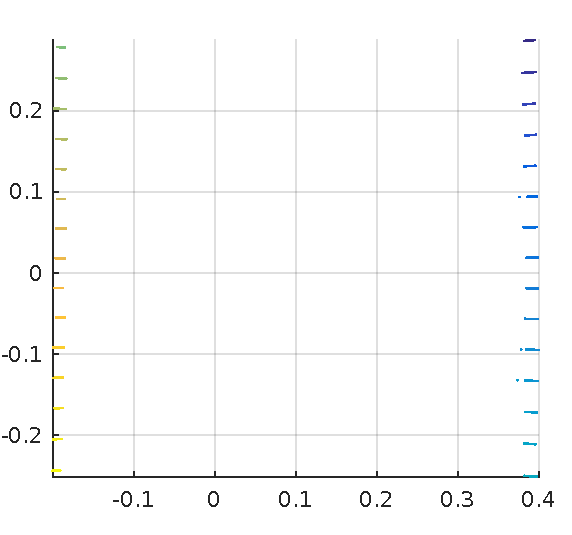
\includegraphics[width=0.21\textwidth]{fig/twoline.pdf}
  }
  \caption{Features in point cloud}
\end{figure}

The four circles are detected by fitting space circle model in edges pointcloud $E_p$ with lines and part of outlies removed.
The feature lines and circles are detected fitting by line model and circle model respectively in the edges point $E_p$,
as shown in Fig.~\ref{fig:circleExtracted} and~\ref{fig:RemovedLines}.
Each time a circle is detected, points within a certain distance to the center of circle was removed from the $E_p$,
then we detect the rest of circle in the remained edge points until all the four circles are found.
After all the circle are locate, the four center points are arranged in the shape of ``Z'' in ascending order as
$c_1, c_2, c_3, c_4$ in Fig.~\ref{fig:Plane3DMarker}.
\begin{equation}
R_{circle} + \delta_1 < norm{(c_i-c_j)} < R_{circle} + \delta_2
\end{equation}
where $(c_i, c_j) = {(1,2), (2,4), (4,3), (3,1)}$; $\delta_1$ and $\delta_2$ are two threshold.
Verification was done by checking distances of circle centres. If verification success,
a rough translation is calculated using equation~(\ref{eq:LargeTranslationZ}) and~(\ref{eq:LargeTranslationXY}).
As RANSAC algorithm is heavily used in this paper, the sketch of RANSAC is given below.

\begin{itemize}
 \item[(1)] Select a random subset of the original data.
 \item[(2)] A model is fitted to the random subset.
 \item[(3)] All other data are then tested against the fitted model.
 \item[(4)] Points that fit the estimated model well are considered as inliers.
 \item[(5)] The estimated model is reasonably good if sufficiently inliers, else the model is rejected.
 \item[(6)] The model is improved by reestimating it using all the inliers.
\end{itemize}

The varieties and implementation of RANSAC can be found in PCL\footnote{\url{http://docs.pointclouds.org/trunk/group__sample__consensus.html}}.

\subsection{Stage II: refine the coarse calibration}
After the initial coarse estimation of the calibration parameters,
the refinement process follows in order to increase the calibration accuracy.
Given a initial calibration, we can project all the 3D edge laser points $P'_i = (X'_i, Y'_i, Z'_i) \in E_l $
onto the image using equation~(\ref{eq:eq1}) and equation~(\ref{eq:eq2}) with consideration of lens distortion:
\begin{equation}
\begin{bmatrix} \leftidx{^c}x_i \\ \leftidx{^c}y_i \\ \leftidx{^c}z_i \end{bmatrix} =
\begin{bmatrix} \mathbf{R} & \mathbf{t} \end{bmatrix}
\begin{bmatrix} X'_i \\ Y'_i \\ Z'_i \\ 1 \end{bmatrix} \\
\label{eq:distortion}
\end{equation}
\[ x_i = \frac{ ^c{x_i} }{^c z_i} ,\quad y_i = \frac{ ^c{y_i} }{^c z_i} \]
\[ x'_i = x_i (1 + k_1 r^2 + k_2 r^4 ) + 2 p_1 x y + p_2(r^2 + 2 x^2) \]
\[ y'_i = y_i (1 + k_1 r^2 + k_2 r^4 ) + p_1 (r^2 + 2 y^2) + 2 p_2 x y \]
\[ u_i = f_xx'_i + c_x, \quad v_i = f_yy'_i + c_y \]
where $r^2_i = x_i^2 + y_i^2$, $k_1$ and $k_2$ are radial distortion coefficients;
$p_1$ and $p_2$ are tangential distortion coefficients. we get those parameters through
camera intrinsic calibration.
$(u_i, v_i)$ just is the projection of point $P'_i$ in the $i$\emph{th} edged image.
In order to reward laser points which hit pixels near edges,
we apply an \emph{Inverse Distance Transform} to the edge image $E_I$;
\begin{equation}
\begin{aligned}
I_c(u, v) = & \alpha E_I(u,v) + \\
(1- & \alpha) \cdot \max_{x,y} E_I(x, y) \cdot \beta^{\sqrt{ (x-v)^2 + (y-v)^2 } }
\label{eq:InverseDistanceTransform}
\end{aligned}
\end{equation}
effectively, this make the cost function smoother to avoid local optima in the search procedure.
where $\max_{x,y} E_I(x, y)$ is a local maximum of $E_I(u, v)$,
Bigger $\alpha$ will increase the strength of the ``edgeness'' its local maximum whereas $\beta$ enlarges the area an edge effectively impacts. 
For ease of the computation, $ \beta^{ \sqrt{ (x-v)^2 + (y-v)^2 } }$ can be instead with
$\beta^{\max\{\lvert x-v \rvert, \lvert y-v \lvert\}}, \beta < 1$,
It it reasonable that the area of effect of local maximum inverse proportion to the distance to it.
\begin{figure}[!ht]
  \centering
  \subfigure[Edge image $E_I$]
  {
    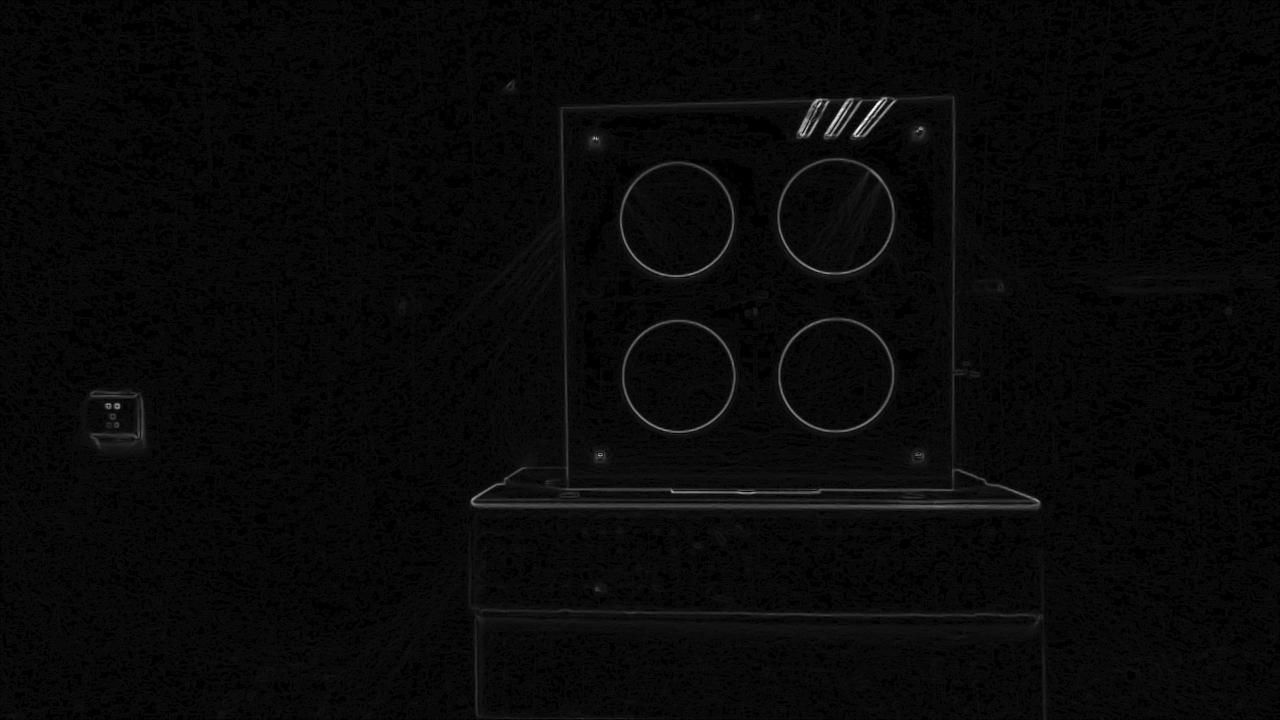
\includegraphics[width=0.4\textwidth]{fig/ImgEdge.JPG}
  }
  \subfigure[Inverse distance transform of $E_I$, denoted as $Ic$:\label{fig:IDTE}]
  {
    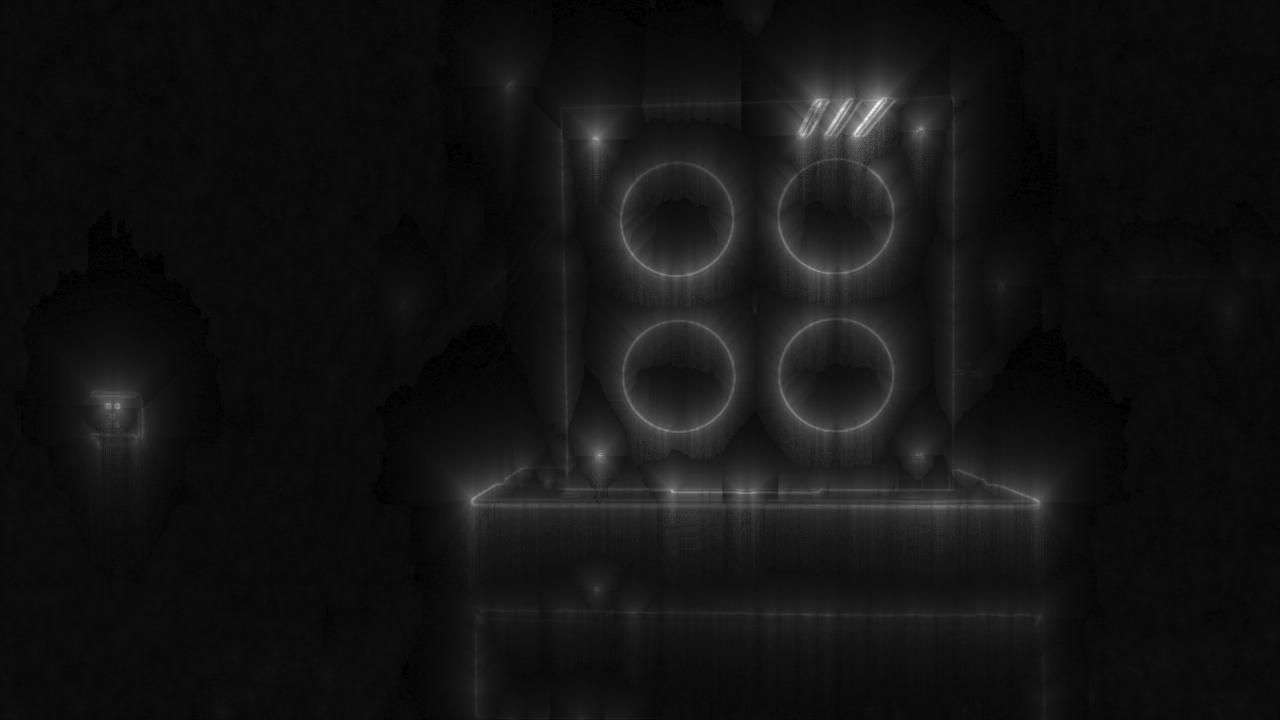
\includegraphics[width=0.4\textwidth]{fig/IDTE2.JPG}
  }
  \caption{One of the original image collected and
  its correspondence Inverse Distance Transform using equation~(\ref{eq:InverseDistanceTransform})}
\end{figure}

If total $N$ pairs of image and velodyne point clouds are observed and there are each that $M$ edge points in the point cloud $E_p$.
We can construct the cost function based on the assumption that
the depth discontinuities in point cloud should match with edges detected in image.
\begin{equation}
\argmax_{\mathbf{R}, \mathbf{t}}{ \sum^N_{j=1} \sum^{M_j}_{i=1} I_{cj}(u_i, v_i) \cdot I_{lj}(X_i, Y_i, Z_i) }
\end{equation}
The above solution is obtained by maximizing the cost function global search of the small subspace of the calibration
parameters around the point of the coarse calibration.


\section{Experimental Results}
Our algorithms were implemented in C++, Fig.~\ref{fig:calib_proj} demonstrates results of calibration.
We do not have precise ground truth, the results look visually good.
The results of calibration is given at Table~\ref{tab:ResultOfExtrinsicCalibration}.
\begin{figure}[!htb]
  \centering
  \subfigure[Manual calibration \label{fig:worse}]
  {
    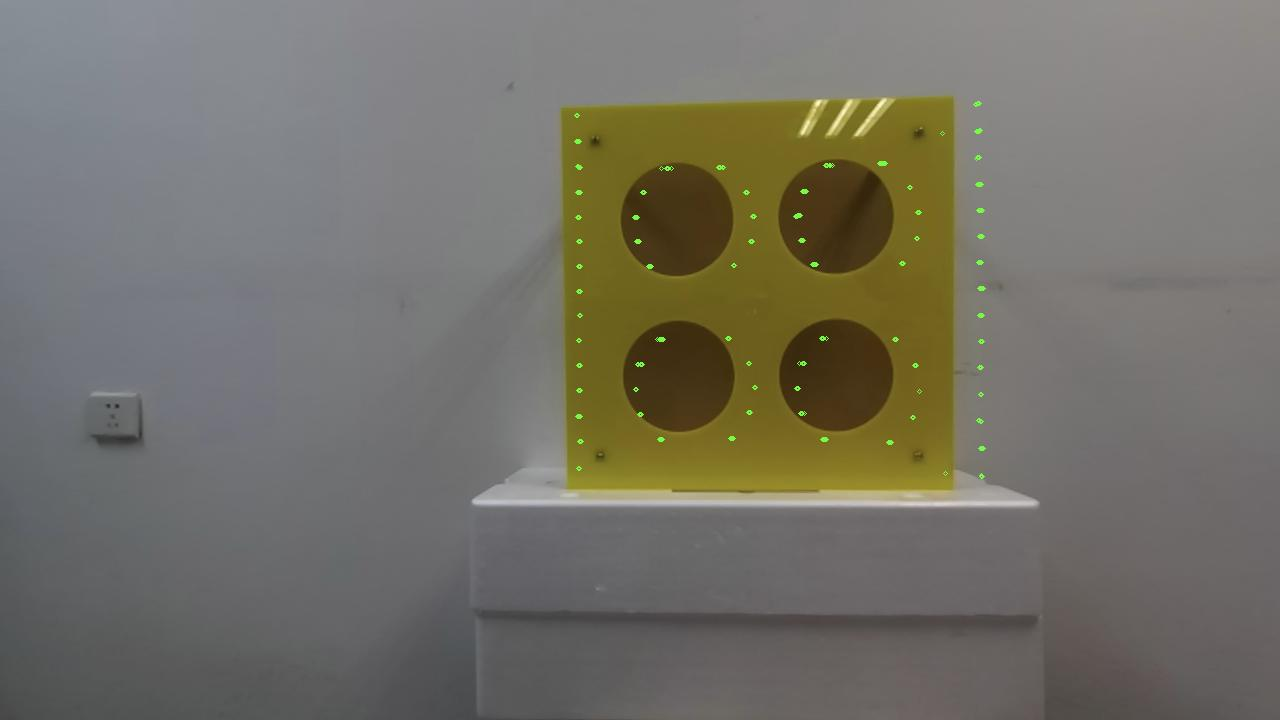
\includegraphics[width=0.44\textwidth]{fig/worse.JPG}
%    \caption{ all edges point to the front plane using the parameters listed in Table~\ref{tab:mannual}}
  }
  \subfigure[After coarse calibration]
  {
    \label{fig:calib_proj:a} %% label for first subfigure
    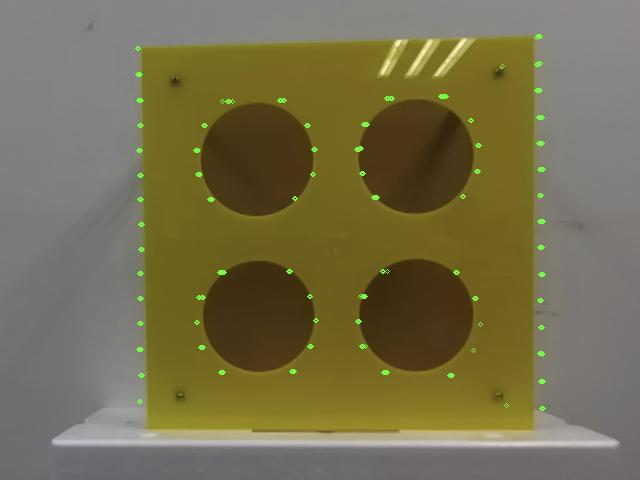
\includegraphics[width=0.22\textwidth]{fig/coarse_calib_proj.jpg}
  }
  \hspace{0.1cm}
  \subfigure[After fined calibration]
  {
    \label{fig:calib_proj:b} %% label for second subfigure
    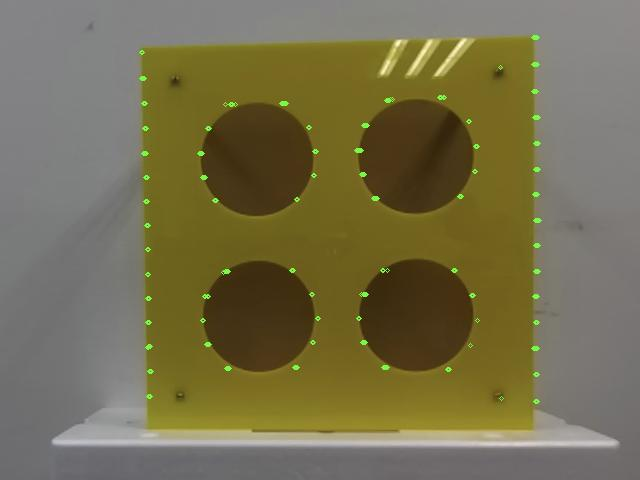
\includegraphics[width=0.22\textwidth]{fig/fine_calib_proj.jpg}
  }
  \caption{Reprojection of the 3D edge points from laser coordinate frame to 2D coodinate frame of the image}
  \label{fig:calib_proj} %% label for entire figure
\end{figure}

\begin{table}[!htb]
  \centering
  \caption{Manual measured extrinsic}
  \label{tab:mannual}
  \begin{tabular}{|c|c|c|c|c|c|}
    \hline
    \multicolumn{3}{|c|}{T(m)} & \multicolumn{3}{c|}{R(rad)} \\ \hline
    $T_x$ & $T_y$ & $T_z$ & $R_x$ & $R_y$ & $R_z$ \\ \hline
    0.07 & -0.06 & -0.02 & 0 & $-\pi/2$ & $ \pi/2 $ \\ \hline
  \end{tabular}
\end{table}

\begin{table}[!htb]
  \centering
  \caption{Results of extrinsic calibration\label{tab:ResultOfExtrinsicCalibration}}
  \label{CoarseCalibration}
  \begin{tabular}{|l|l|l|l|l|l|l|}
    \hline
     &\multicolumn{3}{c}{T(m)} & \multicolumn{3}{|c|}{R(rad)} \\
    \hline
    Method & $T_x$ & $T_y$ & $T_z$ & $R_x$ & $R_y$ & $R_z$ \\ \hline
    coarse & 0.04 & -0.126 & -0.036 & 0 & 0 & 0 \\ \hline
    fine & 0.043 & -0.088 & -0.008 & 0.040 &0.003 &-0.010 \\ \hline
  \end{tabular}
\end{table}

Table~\ref{tab:dataInImage}, ~\ref{tab:dataInPointcloud} give the result of circle detection in image and point cloud respectively.
The units of $(u, v)$ and $ r $ is pixel, expressed in image coordinate.
\begin{table}[!htb]
  \centering
  \caption{Results of circle detection in image\label{tab:dataInImage}}
  \label{CircleInImg}
  \begin{tabular}{|c|c|c|c|c|}
    \hline
    circle2d & c1 & c2 & c3 & c4  \\ \hline
    $(u, v)$ & (676,218) &(838,218) & (678,374) & (836,376) \\ \hline
    $ r(pixel) $  & 57 & 59 & 58 & 58 \\ \hline
  \end{tabular}
\end{table}

\begin{table}[!htb]
  \centering
  \caption{Results of circle detection in point cloud\label{tab:dataInPointcloud}}
  \label{CircleInPointcloud}
  \begin{tabular}{|c|c|c|c|c|}
    \hline
    circle3d & c1 & c2 & c3 & c4  \\ \hline
    $x(m)$ &-0.0195 &-0.0196 & 0.2067 & 0.2111 \\ \hline
    $y(m)$ & 0.1626 &-0.0819 & 0.1622 &-0.0871 \\ \hline
    $z(m)$ & 1.0156 & 1.0219 & 1.0092 & 1.0158 \\ \hline
    $r(m)$ & 0.0841 & 0.0850 & 0.0846 & 0.0833 \\ \hline
  \end{tabular}
\end{table}



\section{Conclusion and Future Work}
This paper presents a pipeline for the RGB camera calibration with Velodyne LiDAR.
The first step in the calibration process estimates a coarse calibration using our novel 3D marker
which allows the large discplacement between the sensors can be roughly estimate using only a single pair of image-point cloud data.
The consequent step refines the coarse calibration using a brute global search in a small 6DoF calibration parameter subspace.
Experment results show the effectiveness of the proposed method.

%\section{Acknowledgements}
%The research leading to these results was funded by the XXX project XXXX (no. TE01020415) 
%The most important evaluation criteria should be the accuracy of calibration results.
%I%\begin{equation}
%\mathbf{R} = Rot(Z, \frac{ \pi }{2} ) \cdot Rot(Y, -\frac{ \pi }{2}) =
%\begin{bmatrix} 0 & -1 & 0  \\ 0 & 0 & -1 \\ 1 & 0  & 0 \end{bmatrix}.
%\end{equation}n stage I, we compute an initial estimate of the transformation by estimating the large translation part independently.

\begin{thebibliography}{0}

\bibitem{ZhangZY200}
Zhang Z. A Flexible New Technique for Camera Calibration, IEEE Transactions on Pattern Analysis \& Machine Intelligence, 2000, 22(11):1330-1334.

\bibitem{Zhang2004}
Zhang Q, Pless R, Extrinsic calibration of a camera and laser range finder (improves camera calibration), in
\emph{IEEE/RSJ International Conference on Intelligent Robots and Systems}, 2004:2301-2306 vol.3.

\bibitem{Unnikrishnan2005}
R. Unnikrishnan and M. Hebert, Fast extrinsic calibration of a laser rangefinder to a camera, Robotics Institute, Pittsburgh, PA, Tech. Rep. CMU-RI-TR-05-09, July 2005.

\bibitem{Geiger2012}
Geiger A, Moosmann F, �0�0 Car, et al, \emph{Automatic camera and range sensor calibration using a single shot} 2012, 20(10):3936-3943.

\bibitem{Scaramuzza2007}
D. Scaramuzza, A. Harit, and R. Siegwart, Extrinsic Self Calibration of a Camera and a 3D Laser Range Finder from Natural Scenes, in
\emph{International Conference on Intelligent Robots and Systems (ICRA)}, 2007.

\bibitem{Rodriguez2008}
Rodriguez F S A, Fremont V, Bonnifait P, Extrinsic calibration between a multi-layer lidar and a camera,
in \emph{IEEE International Conference on Multisensor Fusion and Integration for Intelligent Systems}, IEEE Xplore, 2008:214-219.

\bibitem{Nunez2009}
Nunez P, Jr PD, Rocha R, et al. Data Fusion Calibration for a 3D Laser Range Finder and a Camera using Inertial Data, 2009.

\bibitem{Kassir2010}
Kassir A, Peynot T, In \emph{Proceedings of the 2010 Australasian Conference on Robotics \& Automation}, ACRA2010, Dec 2010.

\bibitem{Pandey2012}
Pandey G, Mcbride J R, Savarese S, et al. Automatic targetless extrinsic calibration of a 3D lidar and camera by maximizing mutual information, 
in \emph{Twenty-Sixth AAAI Conference on Artificial Intelligence}, AAAI Press, 2012:2053-2059.

\bibitem{Taylor2012}
Taylor Z, Nieto J, A Mutual Information Approach to Automatic Calibration of Camera and Lidar in Natural Environments, Acra, 2012.

\bibitem{Levinson2013}
Levinson J, Thrun S, Automatic Online Calibration of Cameras and Lasers, Robotics: Science and Systems, 2013.

\bibitem{Napier2013}
Napier A, Corke P, Newman P, Cross-calibration of push-broom 2D LIDARs and cameras in natural scenes,
in \emph{IEEE International Conference on Robotics and Automation}, 2013:3679-3684.

\bibitem{Moghadam2013}
Moghadam P, Bosse M, Zlot R, Line-based extrinsic calibration of range and image sensors,
in \emph{IEEE International Conference on Robotics and Automation}, 2013:3685-3691.

\bibitem{Velas2014}
M Velas, M Spanel, Z Materna, A Herout, Calibration of RGB Camera With Velodyne LiDAR 
In \emph{WSCG Full Papers Proceedings}, Plzen, 2014, pp. 1-10.

\bibitem{Pandey2014}
Pandey G, Mcbride J R, Savarese S, et al, Automatic Extrinsic Calibration of Vision and Lidar by Maximizing Mutual Information,
Journal of Field Robotics, 2014, 32(5):696-722.

\bibitem{Premebida2014}
Premebida C, Carreira J, Batista J, et al, Pedestrian detection combining RGB and dense LIDAR data, 
in \emph{Ieee/rsj International Conference on Intelligent Robots and Systems}, IEEE, 2014:4112-4117.

\bibitem{Held2012}
Held D, Levinson J, Thrun S, A probabilistic framework for car detection in images using context and scale,
in \emph{IEEE International Conference on Robotics and Automation}, IEEE, 2012:1628-1634.

\bibitem{Held2014}
Held D, Levinson J, Thrun S, et al, Combining 3D Shape, Color, and Motion for Robust Anytime Tracking, Robotics: Science and Systems. 2014.

\bibitem{Bok2013}
Bok Y, Choi D G, Kweon I S, Generalized laser three-point algorithm for motion estimation of camera-laser fusion system,
in \emph{IEEE International Conference on Robotics and Automation}, IEEE, 2013:2880-2887.

\bibitem{Taylor2015}
Taylor Z, Nieto J. Motion-based calibration of multimodal sensor arrays,
in \emph{International Conference on Intelligent Robots and Systems}, 2015:4843-4850.

\bibitem{He2012}
Ha JE, Extrinsic calibration of a camera and laser range finder using a new calibration structure of a plane with a triangular hole,
International Journal of Control, Automation and Systems, 2012, 10(6):1240-1244.

\bibitem{Napier}
Napier A, Corke P, Newman P. Cross-calibration of push-broom 2D LIDARs and cameras in natural scenes,
in \emph{IEEE International Conference on Robotics and Automation}, IEEE, 2013:3679-3684.

\bibitem{Ando2000}
S. Ando, Image field categorization and edge/corner detection from gradient covariance, 
in \emph{IEEE Transactions on Pattern Analysis and Machine Intelligence}, vol. 22, no. 2, pp. 179-190, Feb 2000.

\bibitem{Yuen1990}
Yuen, H. K. and Princen, J. and Illingworth, J. and Kittler, J., Comparative study of Hough transform methods for circle finding.
Image Vision Comput. 8 1, pp 71�C77 (1990)

\bibitem{Canny1986}
J. Canny. A Computational Approach to Edge Detection, IEEE Trans. on Pattern Analysis and Machine Intelligence, 8(6), pp. 679-698 (1986).

\bibitem{RANSAC2000}
Torr P H S, Zisserman A. MLESAC: A New Robust Estimator with Application to Estimating Image Geometry, Computer Vision \& Image Understanding, 2000, 78(1):138-156.

\bibitem{Rusu2011}
Rusu, R.B., Cousins, S. 3D is here: Point Cloud Library (PCL). In \emph{Proceedings of the IEEE International Conference on Robotics and Automation}, Shanghai, China,
9-13 May 2011, pp. 1-4.

\bibitem{Wang2013}
Y. Wang, D. Ewert, D. Schilberg and S. Jeschke, Edge extraction by merging 3D point cloud and 2D image data,
in \emph{2013 10th International Conference and Expo on Emerging Technologies for a Smarter World (CEWIT)}, Melville, NY, 2013, pp. 1-6.

\bibitem{Mach1981}
Fischler, M.A., Bolles, R.C. Random Sample Consensus: A paradigm for model fitting with applications to image analysis and automated cartography.Commun. ACM. 1981,24,381-395

\end{thebibliography}

\end{document}
